%% paper preamble
\documentclass[10pt,a4paper, twocolumn]{article}

\usepackage[utf8]{inputenc}
\usepackage[german]{babel}
\usepackage[T1]{fontenc}
\usepackage{fullpage}
\usepackage{graphicx}
\usepackage{listings}
\usepackage{tcolorbox}
\usepackage{url}
\usepackage{float}
\usepackage{nameref}
%\usepackage{subcaption}
\usepackage{hyperref}
\usepackage{xcolor}

\hypersetup{
  colorlinks   = true, 	%Colours links instead of ugly boxes
  urlcolor     = red, 	%Colour for external hyperlinks
  linkcolor    = blue, 	%Colour of internal links
  citecolor   = blue 	%Colour of citations
}
\definecolor{grey}{rgb}{0.9,0.9,0.9}

\setlength{\parindent}{0pt}
\setlength{\columnsep}{0.5cm}


\usepackage{amsmath}
\usepackage[]{algorithm2e}
\usepackage[]{csquotes}
\usepackage{subfigure}

\author{Sven Fiergolla \\ 1252732 \\ s4svfier@uni-trier.de}
\title{Index Construction}

\hypersetup{
    colorlinks=true,
    linkcolor=black,
    urlcolor=blue
}

\begin{document}

\LinesNumbered
\maketitle

\section{Einführung}
\paragraph{}
Information Retrieval, zu deutsch Informationsrückgewinnung, ist ein Fachgebiet, welcher sich mit computergestütztem Suchen nach komplexen Inhalten befasst. Der häufigste Anwendungsbereich ist das Suchen von Dokumenten aus einer Sammlung, die für einen Anwender relevant sind. Würde dies auf der unveränderten Datenmenge geschehen, müsste bei jeder Suchanfrage, die komplette Menge an Rohdaten durchsucht werden. Dies ist ein sehr ressourcenintensiver Prozess, daher wird zunächst auf die Hardware sebst eingegangen. Anschließend werden einige Verfahren zum Erstellen eines Index vorgestellt und auf deren Vor- und Nachteile eingegangen.\par

\section{Hardware Constraints}
\begin{figure*}[ht]
  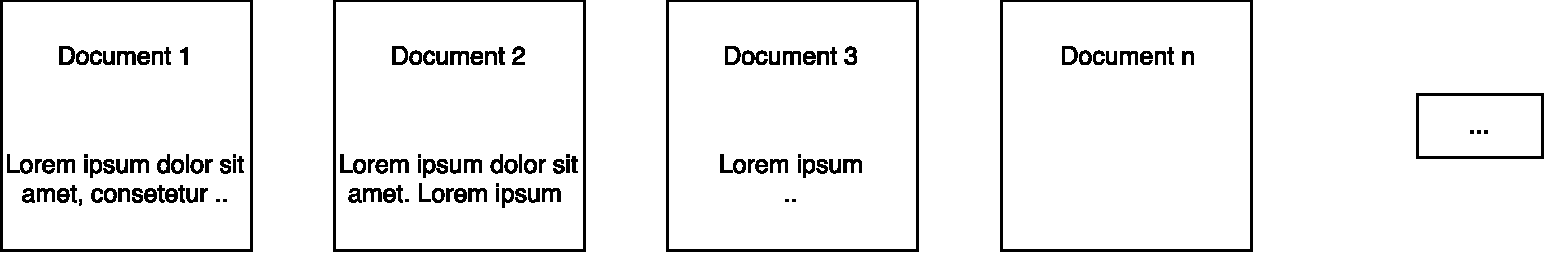
\includegraphics[width=\textwidth]{pdf/Documents.pdf}
  \caption{beispielhafter Dokumenten-Korpus}
  \label{korpus}
\end{figure*}

\paragraph{}
Typische Systemeigenschaften eines Desktop PC im Consumerbereich (Stand 2018):
\begin{itemize}
	\item \textit{clock rate} 2-4 GHz, 4-8 Kerne
	\item \textit{main memory} 4-32 Gb
	\item \textit{disk space} $\leq$ 1 TB SSD oder $\geq$ 1 TB HDD
	\begin{itemize}
	\item HDD (hard disk drive)
	\begin{itemize}
	\item \textit{average seek time} zwischen 2 und 10 ms
	\item \textit{transfer} 150 - 300 MB/s
	\end{itemize}
	\item SSD (solid state disk)
	\begin{itemize}
	\item \textit{average seek time} zwischen 0.08 und 0.16 ms
	\item \textit{transfer} Lesen: 545 MB/s, Schreiben: 525 MB/s
	\end{itemize}
	\end{itemize}
\end{itemize}	 
\par

\paragraph{}
Die zu durchsuchende Datensammlung, häufig auch Korpus geannt, befindet sich auf der Festplatte, welche deutlich langsamer arbeitet als der Arbeitsspeicher oder die CPU. Daher stellt die Festplatte in diesem Fall ein Bottleneck\footnote{Wörtlich: \enquote{Flaschenhals} oder \enquote{Engpass}. Gemeint ist ein Engpass beim Transport von Daten, der maßgeblichen Einfluss auf die Arbeitsgeschwindigkeit hat.} dar.
Um die intensive Nutzung der Festplatte zu vermeiden, wird eine alterntive Datenstruktur benötigt. Je nach Anforderung kann eine andere Struktur verwendet werden. Für klassisches \enquote{Document Retrival} wird jedoch in der Regel ein so genannter Invertiert Index konstruiert (siehe \nameref{invertedIndex}).
Da sich mit der SSD eine neue Speichertechnologie verbreitet hat, welche deutlich bessere Zugriffszeiten hat als eine HDD, wird diese seperat betrachtet (siehe \nameref{indexSSD}).
\par

\section{Index Construction} \label{IndexConstruction}
\paragraph{}
Um das ressourcenintensive Durchsuchen der Rohdaten zu vermeiden, existieren geeignete Datenstrukturen um Anfragen beantworten zu können, ohne alle Daten durchsuchen zu müssen. Eine einfache geeignete Struktur wäre eine \enquote{Term-Dokument-Matrix}, welche spaltenweise die Dokumente auflistet und zeilenweise das Vorkommen einzelner Worter. Auf einer solchen Matrix lässts sich mit einfachen boolschen Anfragen arbeiten, jedoch hat diese Datenstruktur auch einige Nachteile. Beipsielsweise wächst die Matrix zu stark an für große Sammlungen, es lassen sich keine Komplexeren Anfragen stelle und ein Ranking der Dokumente ist ebenfalls nicht möglich. Daher betrachten wir im Folgenden lediglich den invertierten Index als geeignete Datenstruktur.
\par

\paragraph{}
Um aus einer Sammlung von Rohdaten (Abbildung \ref{korpus}) die relevanten Informationen zu gewinnen, müssen vorher einige Anpassungen getätigt werden. Besteht die Sammlung beispielsweise aus Webseiten, müssen die Informationen vor dem Indizieren aus der \textit{.html}-Datei geparst und von html-Tags befreit werden. In der Regel wird ebenfalls Tokenization und Stemming auf den Text angewendet. Bei der Tokenisierung wird Dokument in kleinste Einheiten (meistens einzene Wörter) geteilt. Stemming erlaubt, dass verschiedene morphologische Varianten eines Wortes auf ihren gemeinsamen Wortstamm zurückgeführt werden (beispielsweise die Deklination von Wortes oder Wörter zu Wort und Konjugation von gesehen oder sah zu seh). Dies ermöglicht, dass bei einer Suchanfrage auch Dokumente gefunden werden können, in denen eine leichte Variation des gesuchten Wortes vorkommt, da beide auf den gleichen Term reduziert werden.
\par

\subsection{Invertierter Index} \label{invertedIndex}
\paragraph{}
Die wesentlichen Schritte zur Erstellung eines invertierten Index sind in Abbildung \ref{postingssList} dargestellt. Zuerst werden alle \enquote{Term-Dokument ID} Paare gesammelt. Diese werden anschließend, dem Term nach, lexikographisch sortiert. Zuletzt werden die Dokument ID's für jeden Term in einer so genannten Postingslist zusammengefasst und Statistiken wie die Frequenz eines Terms berechnet. Die Postingslisten aller Terme bezeichnet man als invertierten Index, da die Zuordnung von Dokumenten auf deren Text invertiert wurde zu der Zuordnung zwischen einem Term und dessen Vorkommen. Bei einer Suchanfrage muss nun lediglich die Postingsliste zu dem gesuchten Term zurückgegeben werden. Aus Performancegründen werden häufig eindeutige Term ID's statt den Termen selbst genutzt. Für kleine Sammlungen kann dies im Arbeitsspeicher geschehen, für größere Sammlungen werden jedoch alternative Verfahren benötigt, auf die im Folgenden eingegangen wird.
\par

\begin{figure*}[ht]
  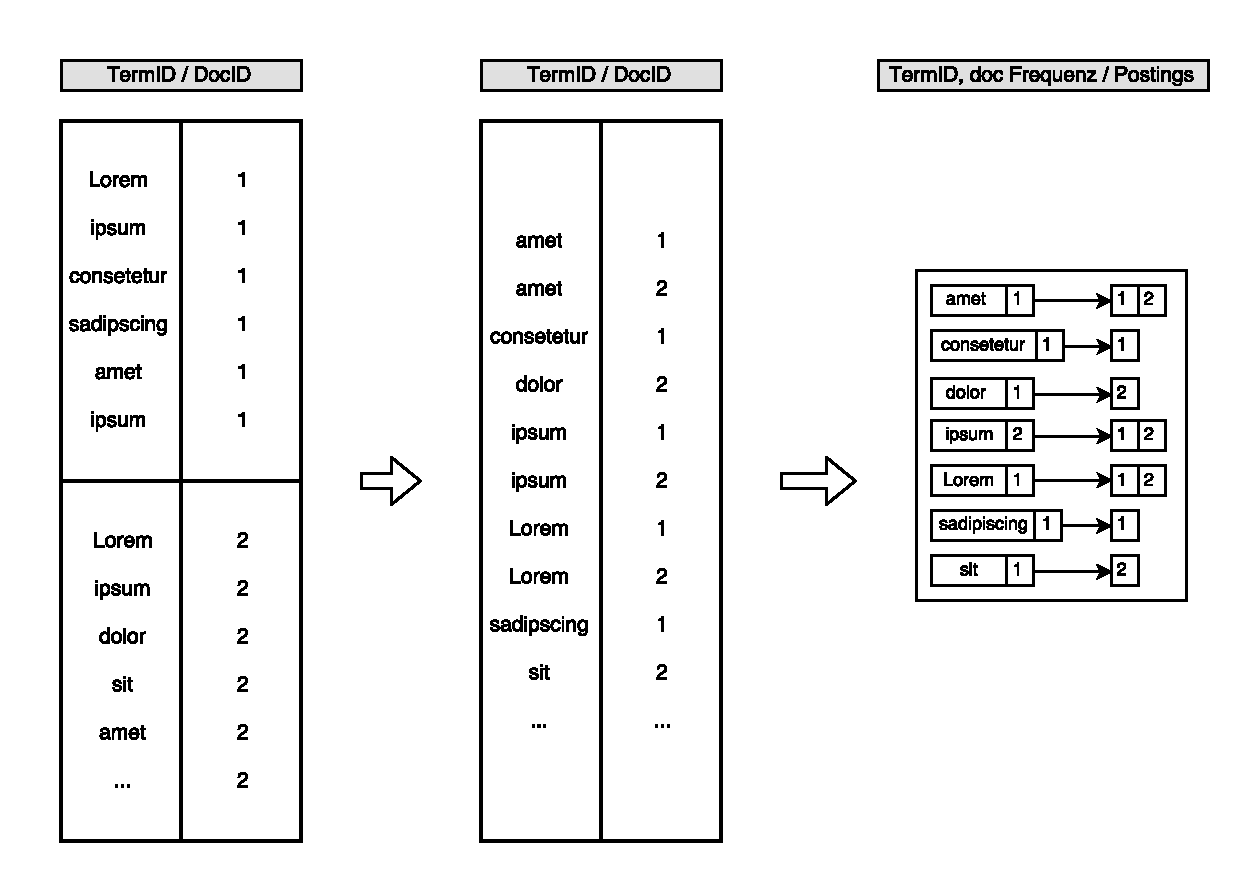
\includegraphics[width=\textwidth,height=0.4\textheight]{pdf/postingslist3.pdf}
  \caption{Invertierter Index}
  \label{postingssList}
\end{figure*}

\paragraph{}
In \enquote{Introduction to Information Retrieval}\cite{ir} wird beispielhaft mit einer Modelsammlung gearbeitet, der Reuters-RCV1. Sie umfasst rund $800.000$ Nachrichtenartikel, ist etwa 1 GB groß und besitzt $100.000.000$ Terme. Die \enquote{Term-Dokument ID} Paare dieser Sammlung auf einer Festplatte zu sortieren ist sehr ineffizient. Beim Sortieren kann von einer Komplexität von $O(n \cdot log_2 (n))$ ausgegangen werden. Möchte man nun alle Terme der Reuters-RCV1 Sammlung sortieren und man von 2 Zugriffen auf die Festplatte beim Sortieren sowie einer durchschnittlichen Zugriffszeit auf die Festplatte von 5ms ausgeht, dauert es in etwa:

\[(100.000.000 \cdot log_2 (100.000.000)) \cdot 2 \cdot (5 \cdot 10^{-3}) \]
\[ = 2.6575424759... \cdot 10^7 \text{ Sekunden}\]
\[ = 307.59 \text{ Tage} \]

Diese Dauer resultiert vorallem aus der hohen Zugriffszeit einer mechanischen Festplatte, da bei jedem wahlfreiem Zugriff der Lesekopf neu positioniert werden muss. Das Lesen von sequenziellen Daten ist deutlich schneller. Ein erster Ansatz ist es, den wahlfreien Zugriff zu minimieren und die Daten hauptsächlich Blockweise zu lesen.
\par

\subsection{Blocked sort-based indexing}
\paragraph{}
Eine Ansatz dies zu umgehen ist den Index Blockweise zu erstellen mit Hilfe des \textit{block sort-based indexing Algorithmus} (siehe Algorithmus \ref{bsbiAlgo}) oder auch \textit{BSBI} auf welchen im Folgenden näher eingegangen wird.
\par
\begin{algorithm}
 n = 0\;
 \While{all documents have not been processed}{
n = n + 1\;
block = ParseNextBlock()\;
BSBI-INVERT(block)\;
WriteBlockToDisk(block, $f_n$)\;
  }
  MergeBlocks($f_1$, $\cdots$, $f_n$; $f_{merged}$)\;
\caption{BSBI Algorithmus} \label{bsbiAlgo}
\end{algorithm}

\paragraph{}
Der Algoritmus parst eine Menge von Dokumeten in \enquote{Term-Dokument ID} Paare bis ein Block mit einer festen Größe voll ist (Zeile 4). Anschließend wird der Block sortiert, daher sollte der Block problemlos in den Arbeitsspeicher passen, da dieser wesentlich schneller arbeitet als die Festplatte und so ein effizienteres Sortieren ermöglicht wird. Nun wird ein invertierter Index für den Block erstellt und persistiert (Zeile 5). Dies geschieht iterativ für alle Blöcke bis die Sammlung komplett bearbeitet wurde. Zuletzt werden die einzelnen Postingslist zusammengefügt (Zeile 8) bis alle Listen in einen Invertierten Index über alle Dokumente gemerged wurden (siehe Abbildung \ref{bsiMerging}). 
\par

\begin{figure*}[ht]
  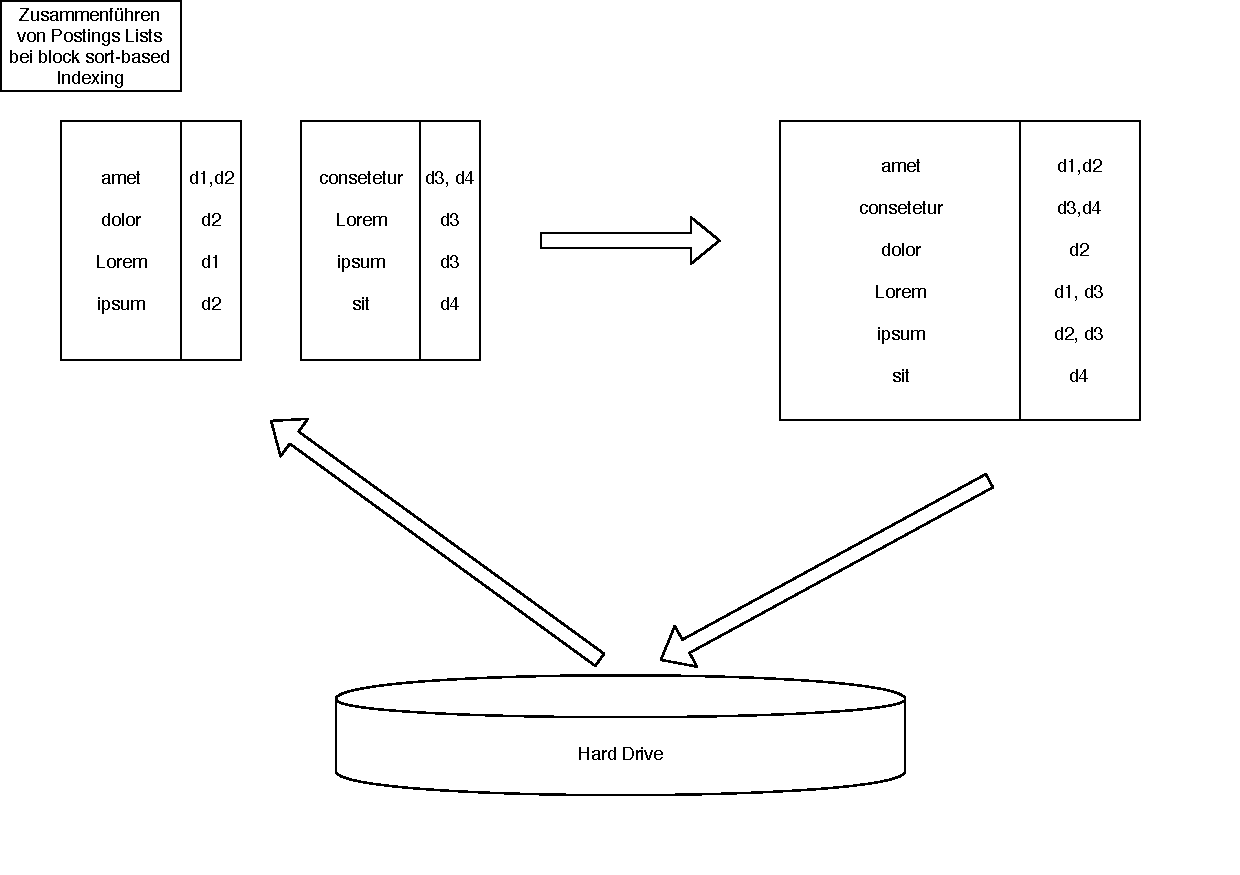
\includegraphics[width=\textwidth]{pdf/BSI_merging.pdf}
  \caption{merging bei BSBI}
  \label{bsiMerging}
\end{figure*}

\paragraph{}
Soll über die Reuters-RCV1 Sammlung mit BSBI ein Index erstellt werden, so dauert dies unter gleichen Voraussetzungen nur noch 15,5 Stunden, da die Sammlung in 64 Blöcke aufgeteilt wird. Diese können innerhalb des Arbeitsspeichers sortiert werden, welcher eine wesentlich bessere Zugriffsgeschwindigkeit vorweist. Dennoch ist die theoretische Zeitkomplexität von BSBI $\Theta( T log_2 ( T))$ da die $T$ Terme sortiert werden müssen, auch wenn dies innerhalb eines Blocks geschieht. In der Praxis ist jedoch meistens das Parsen und Mergen der Blöcke am zeitaufwendigsten. Zudem wird mit Term-ID's gearbeitet,  daher muss zusätzlich eine Datenstruktur für das Mapping zwischen Termen und Term-ID's im Arbeitsspeicher gehalten werden.\par

\subsection{Single-pass in-memory indexing}
\paragraph{}
BSBI lässt sich für viele Sammlungen anwenden, benötigt jedoch eine Datenstruktur für das Mapping zwischen Termen und ihren Term-ID's. Eine alternative Umsetzung ist der \textit{single-pass in-memory indexing Algorithmus} oder auch \textit{SPIMI} (siehe Algorithmus \ref{spimiAlgo}). Anders als bei BSBI werden bei SPIMI Terme statt Term-ID's betrachtet, daher kann auf ein Mapping wie bei BSBI verzichtet werden. Zudem werden die Terme in einem Dictionary gehalten und beim Auftreten der Postingslist angehangen, sodass auf das Sortieren der Terme verzichtet werden kann. Das Dictionary ist eine einfach geordnete Datenstruktur für das Mapping zwischen einem Term und dessen Hash, welche für jeden Block seperat erstellt wird.\par

\paragraph{}
 Die Sammlung von Dokumenten wird als Datenstrom\footnote{Als Datenstrom (Englisch: data streams) bezeichnet man einen kontinuierlichen Fluss von Datensätzen, dessen Ende meist nicht im Voraus abzusehen ist.} von \enquote{Term-Dokument ID} Paaren betrachtet und darauf wiederholt der Algorithmus angewendet, bis die ganze Sammlung indiziert wurde. Wenn ein Term innerhalb eines Bocks zum ersten mal vorkommt, wird er dem Dictionary hinzugefügt (Zeile 6, Abbildung \ref{fig:subfigure1}) und eine neue Postingsliste wird erstellt. Kommt ein Term wiederholt vor, so wird über das Hash des Dictionary auf die Postingsliste zugegriffen (Zeile 8, Abbildung \ref{fig:subfigure2}) und das neue Vorkommen als Posting der Liste hinzugefügt. Da die Länge der Postingsliste nicht dynamisch ist, muss sie bei Bedarf verdoppelt werden (Zeile 11). Wenn der verfügbare Arbeitsseicher verbraucht ist, wird das Dictionary und die Postingslisten des Blocks persistiert und ein neuer Block geparst und bearbeitet (Zeile 17). Die Terme müssen sortiert im Dictionary vorliegen, da die Postingslisten dann in lexikoraphischer Ordnung persistiert werden können. Wurden alle Blöcke bearbeitet, werden die einzelnen Postingslisten zusammengeführt. Dies ist deutlich effizienter wenn sich die Postingslisten der einzelnen Blöcke bereits in lexikographischer Ordnung befinden.\par

\paragraph{}
%TODO
todo fazit\par

\subsection{Distributed indexing}
\paragraph{}
BSBI und SPIMI eignen sich gut für Datensammlungen, die von einem Rechner verarbeitet werden können. Übersteigt der Umfang der Sammlung jedoch die Rechenleistung eines einzelnen Rechners, muss auf andere Weise herangegangen werden. Das Web umfasst ca eine Millarden Webseiten und muss daher von einem Computer-Cluster bearbeitet werden. Ein Computercluster oder Rechnerverbund bezeichnet eine Menge von vernetzten Computern. Solche Cluster bieten die Möglichkeit eine \textit{MapReduce}-Architektur anzuwenden, eine generelle Architektur für verteiltes Arbeiten. So können aufwendige Probleme von vielen, günstigen Rechnern, auch \textit{Nodes} genannt, gelöst werden. Ein einzelner Rechner wird zum \textit{Master-Node}, welcher für das Verteilen der einzelnen Aufgaben verantwortlich ist. Da einzelne Nodes jederzeit ausfallen können, muss der Master-Node Aufgaben jederzeit neu zuweisen können.\par

\paragraph{}
Wird ein Index auf einem solchen verteiltem System erstellt, ist auch der Index selbst geteilt (siehe \nameref{distribIndex}). Dies geschieht entweder nach Dokumenten oder nach Termen. Wird der Index nach Dokumenten geteilt, bearbeiten unterschiedliche Maschinen des Clusters unterschiedliche Abschnitte der Sammlung und erstellen einen Index für jeden Abschnitt welche abschließend zusammengeführt werden. Häufig wird der Index jedoch auch nach Termen geteilt, diese Herangehensweise wird im Folgenden näher beschrieben. Da der Index verteilt erstelt wird, ist auch die Zuordnung zwischen Termen und ihren Term-ID's verteilt und daher komplexer. Eine einfache Lösung ist es, die Zuordnung für häufige Terme im Voraus zu berechnen und auf alle Nodes zu verteilen. Für seltene Terme können die Terme statt Term-ID's verwendet werden.\par

\paragraph{}
Zu Beginn wird die Sammlung in $n$ gleiche Teile unterteilt, die sogenannten \textit{Splits}. Ein Ansatz ist es, die Anzahl der Splits gleich der Anzahl an Nodes zu wählen, so kann jedem Node genau ein Split zugeordnet werden. Alternativ sollte die Größe eines Splits so gewählt werden, dass die Arbeit gleich verteilt werden kann und ein Split von einem herkömmlichen Rechner in einer kurzen Zeit bearbeitet werden kann (16 oder 64MB pro Split). Während der ersten Phase von MapReduce, der \textit{Map-Phase} wird jedem Node ein Split zugewiesen und geparst. Die Ausgabe der $r$ Nodes wird in $j$ lokale Hilfsdateien gespeichert, welche auch \textit{segment files} genannt werden. Sie beinhalten die Postings je einen von mehreren lexikographischen Abschnitt von Termen eines Splits, was es ermöglicht diese später sequenziell auszulesen. In der \textit{Reduce-Phase} weist der Master-Node je einen der $j$ lexikographischen Abschnitte einem Node zu, welcher alle $r$ segment files dieses Abschnittes zusammenführt. Abschließend werden die verbundenen und sortierten Postingslisten persistiert (siehe \enquote{postings} in Abbildung \ref{distribIndex}).\par

\subsection{Dynamic indexing}
\paragraph{}


\subsection{andere Indexierungsverfahren}



\section{Indexierung mit Solid State Drives} \label{indexSSD}

\section{Fazit}

\begin{thebibliography}{9}

		\bibitem{ir}
		Christopher D. Manning, Prabhakar Raghavan and Hinrich Schütze \enquote{\href{https://nlp.stanford.edu/IR-book/pdf/04const.pdf}{Introduction to Information Retrieval}}  Cambridge University Press 2008, pp. 1-18 and 67-84.

	 \bibitem{managigGig}
	  Ian H. Witten, Alistair Moffat, Timothy C. Bell \enquote{\href{https://books.google.de/books?id=2F74jyPl48EC&dq=Witten+et+al.+index+1999&lr=&hl=de&source=gbs_navlinks_s}{Managing Gigabytes: Compressing and Indexing Documents and Images}}  Morgan Kaufman Publishers 1999, pp. 223-261.
	
	\bibitem{ssd}
	Yinan Li, Bingsheng He, Robin Jun Yang, Qiong Luo, Ke YiTree (Hong Kong University of Science and Technology) \enquote{\href{http://pages.cs.wisc.edu/~yinan/paper/fdtree_pvldb.pdf}{Indexing on Solid State Drives}} The 36th International Conference on Very Large Data Bases, September 13-17,
2010, Singapore.
\end{thebibliography}

\newpage

\section*{Appendix}
\subsubsection*{Single-pass in-memory indexing Algorithmus}

\begin{algorithm}
\emph{SPIMI-Invert(token\_ stream)}\\
 outputFile = new File()\;
 dictionary = new HashFile()\;
 \While{free memory available}{
 token = next(TokenStream)\;
\eIf{term(token) $\notin$ dictionary}{
PostingsList = AddToDictionary(dictionary, term(token))\;
}{
PostingsList = GetPostingsList(dictionary, term(token))\;
}
\If{full(PostingsList)}{
PostingsList = DoublePostingsList(dictionary, term(token))\;
}
AddToPostingsList(PostingsList, docID(token))\;
  }
SortedTerms = SortTerms(dictionary)\;
WriteBlockToDisk(SortedTerms, dictionary, OutputFile)\;

  \caption{SPIMI-invert Algorithmus} \label{spimiAlgo}
\end{algorithm}

\pagebreak
\newpage


\begin{figure*}[ht]
       \subfigure{
            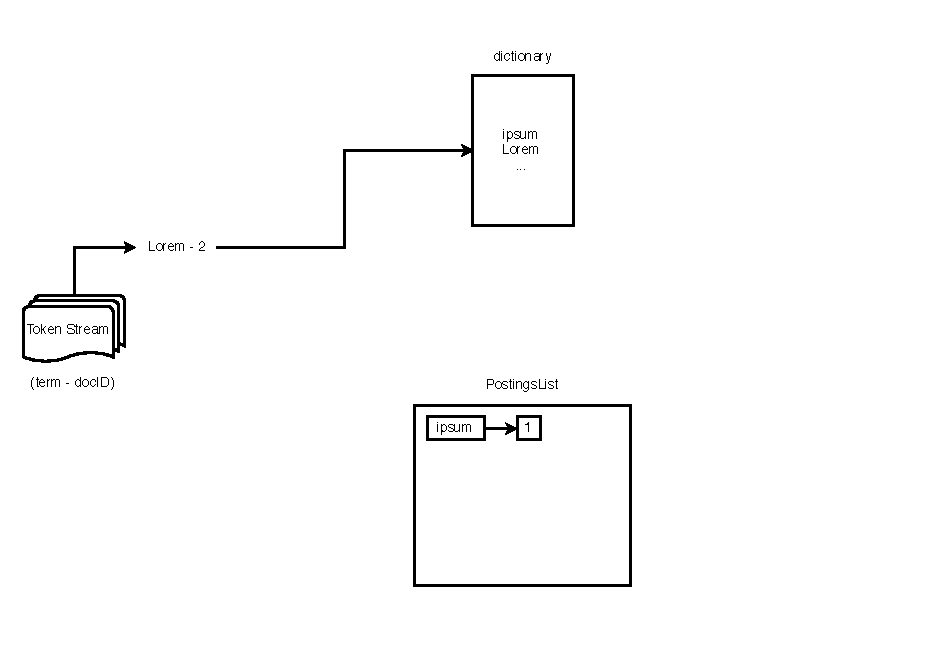
\includegraphics[height=.46\textheight]{pdf/spimi3.pdf}
        }
        \subfigure{
           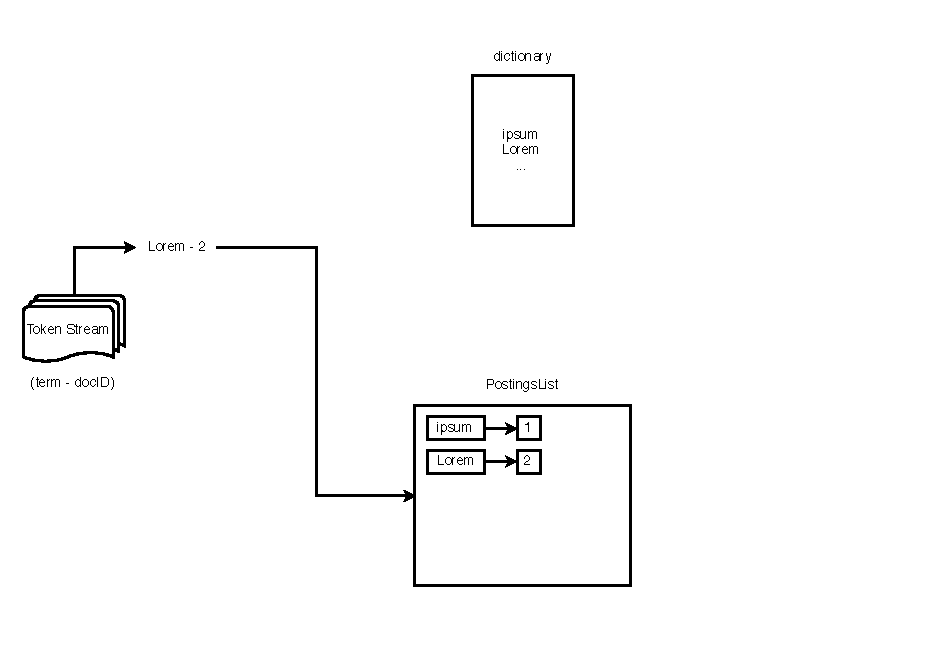
\includegraphics[height=.46\textheight]{pdf/spimi4.pdf}
        }
    \caption{
        Erstes Auftreten eines Terms. Term wird Dictionary hinzugefügt und Postingsliste wird erstellt.
     }
   \label{fig:subfigure1}
\end{figure*}


\begin{figure*}[ht]
        \subfigure{
            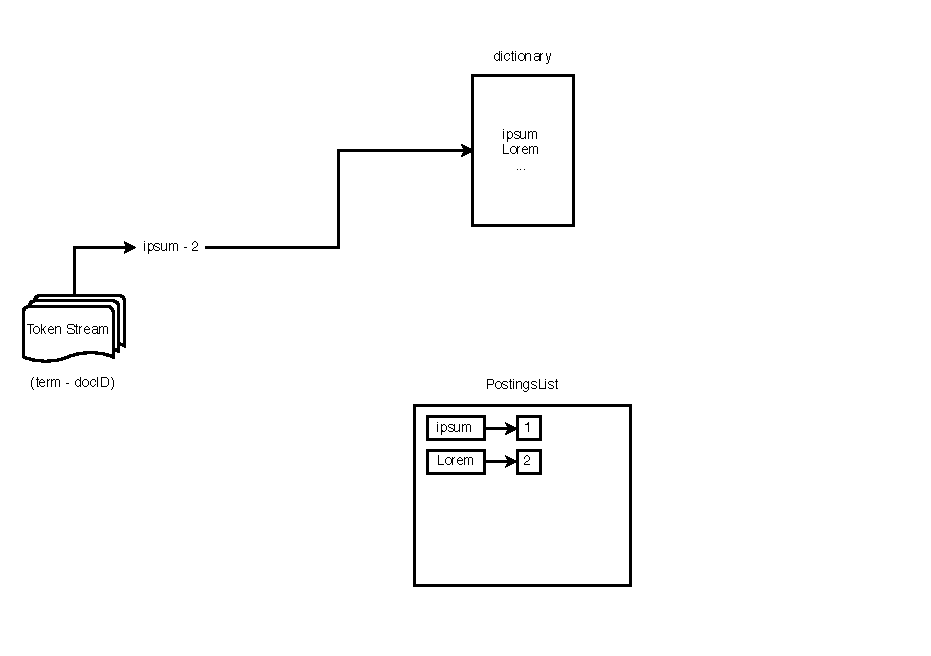
\includegraphics[height=.46\textheight]{pdf/spimi6.pdf}
        }
        \subfigure{
           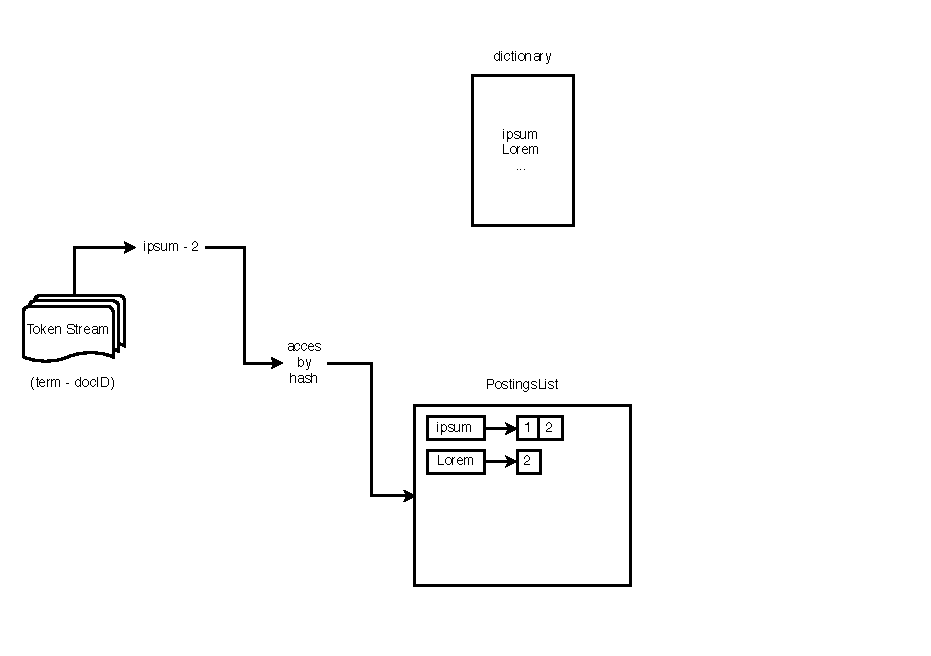
\includegraphics[height=.46\textheight]{pdf/spimi7.pdf}
        }
    \caption{
        Wiederholtes Auftreten eines Terms. Term wird in Dictionary gefunden und per Hash der Postingsliste des Terms hinzuefügt.
     }
   \label{fig:subfigure2}
\end{figure*}

\begin{figure*}[hb]
  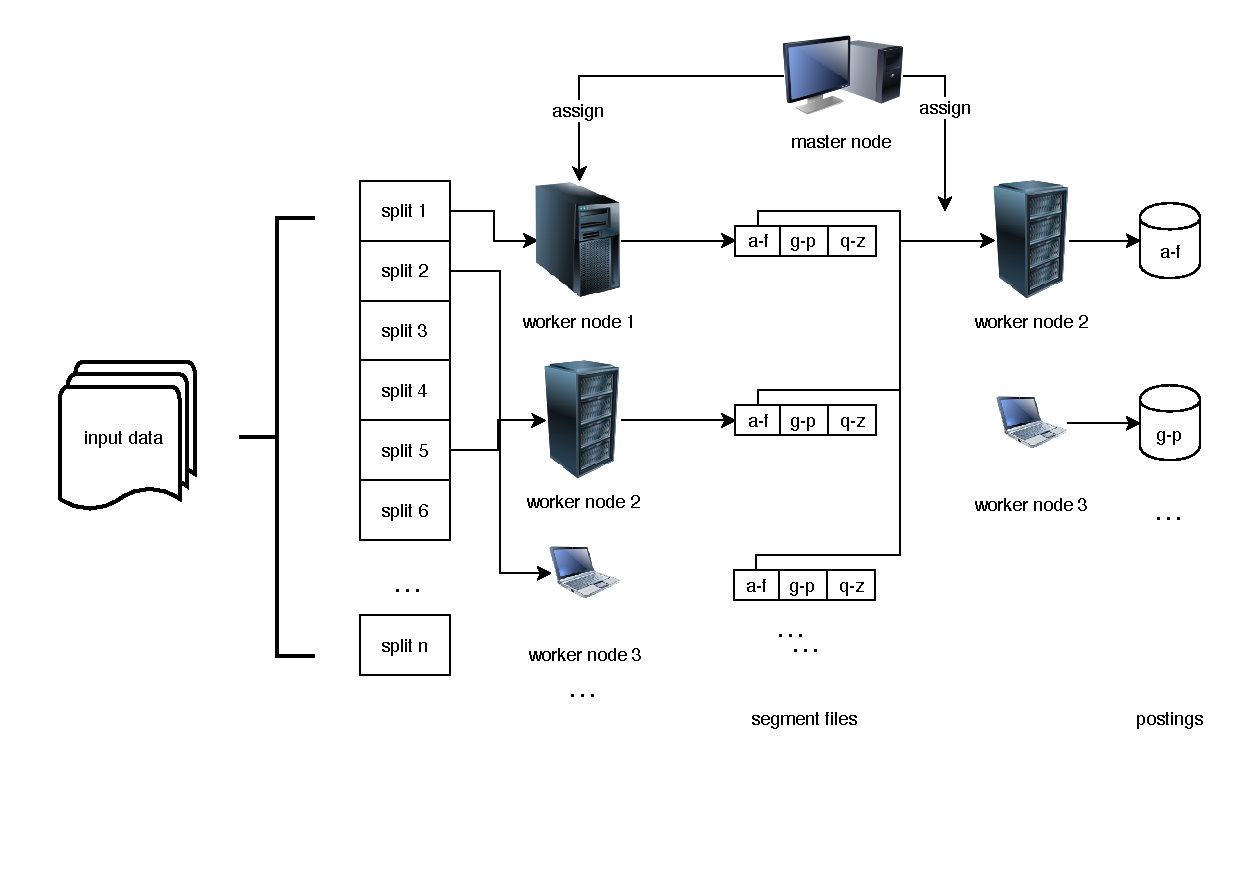
\includegraphics[width=\textwidth]{pdf/distributedIndexAll.pdf}
  \caption{distributed indexing mit MapReduce}
  \label{distribIndex}
\end{figure*}

\begin{figure*}[hb]
  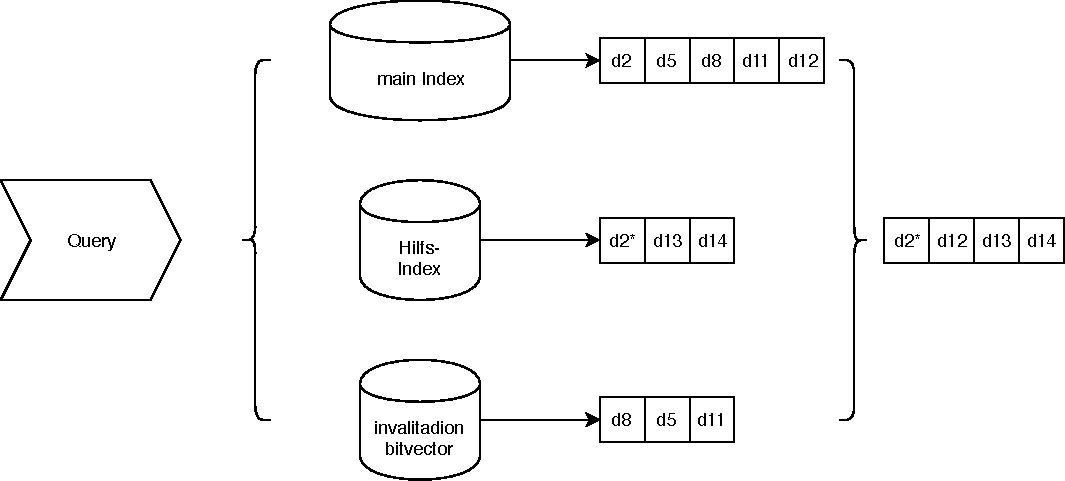
\includegraphics[width=\textwidth]{pdf/dynamicindex.pdf}
  \caption{Query auf einem dynamic index}
  \label{dynIndex}
\end{figure*}
\end{document}